% !TEX root = MutationTestingSurvey.tex

\section{Mutation Testing Process}
\label{sec:dataProcess}

	\begin{figure}
	\centering
		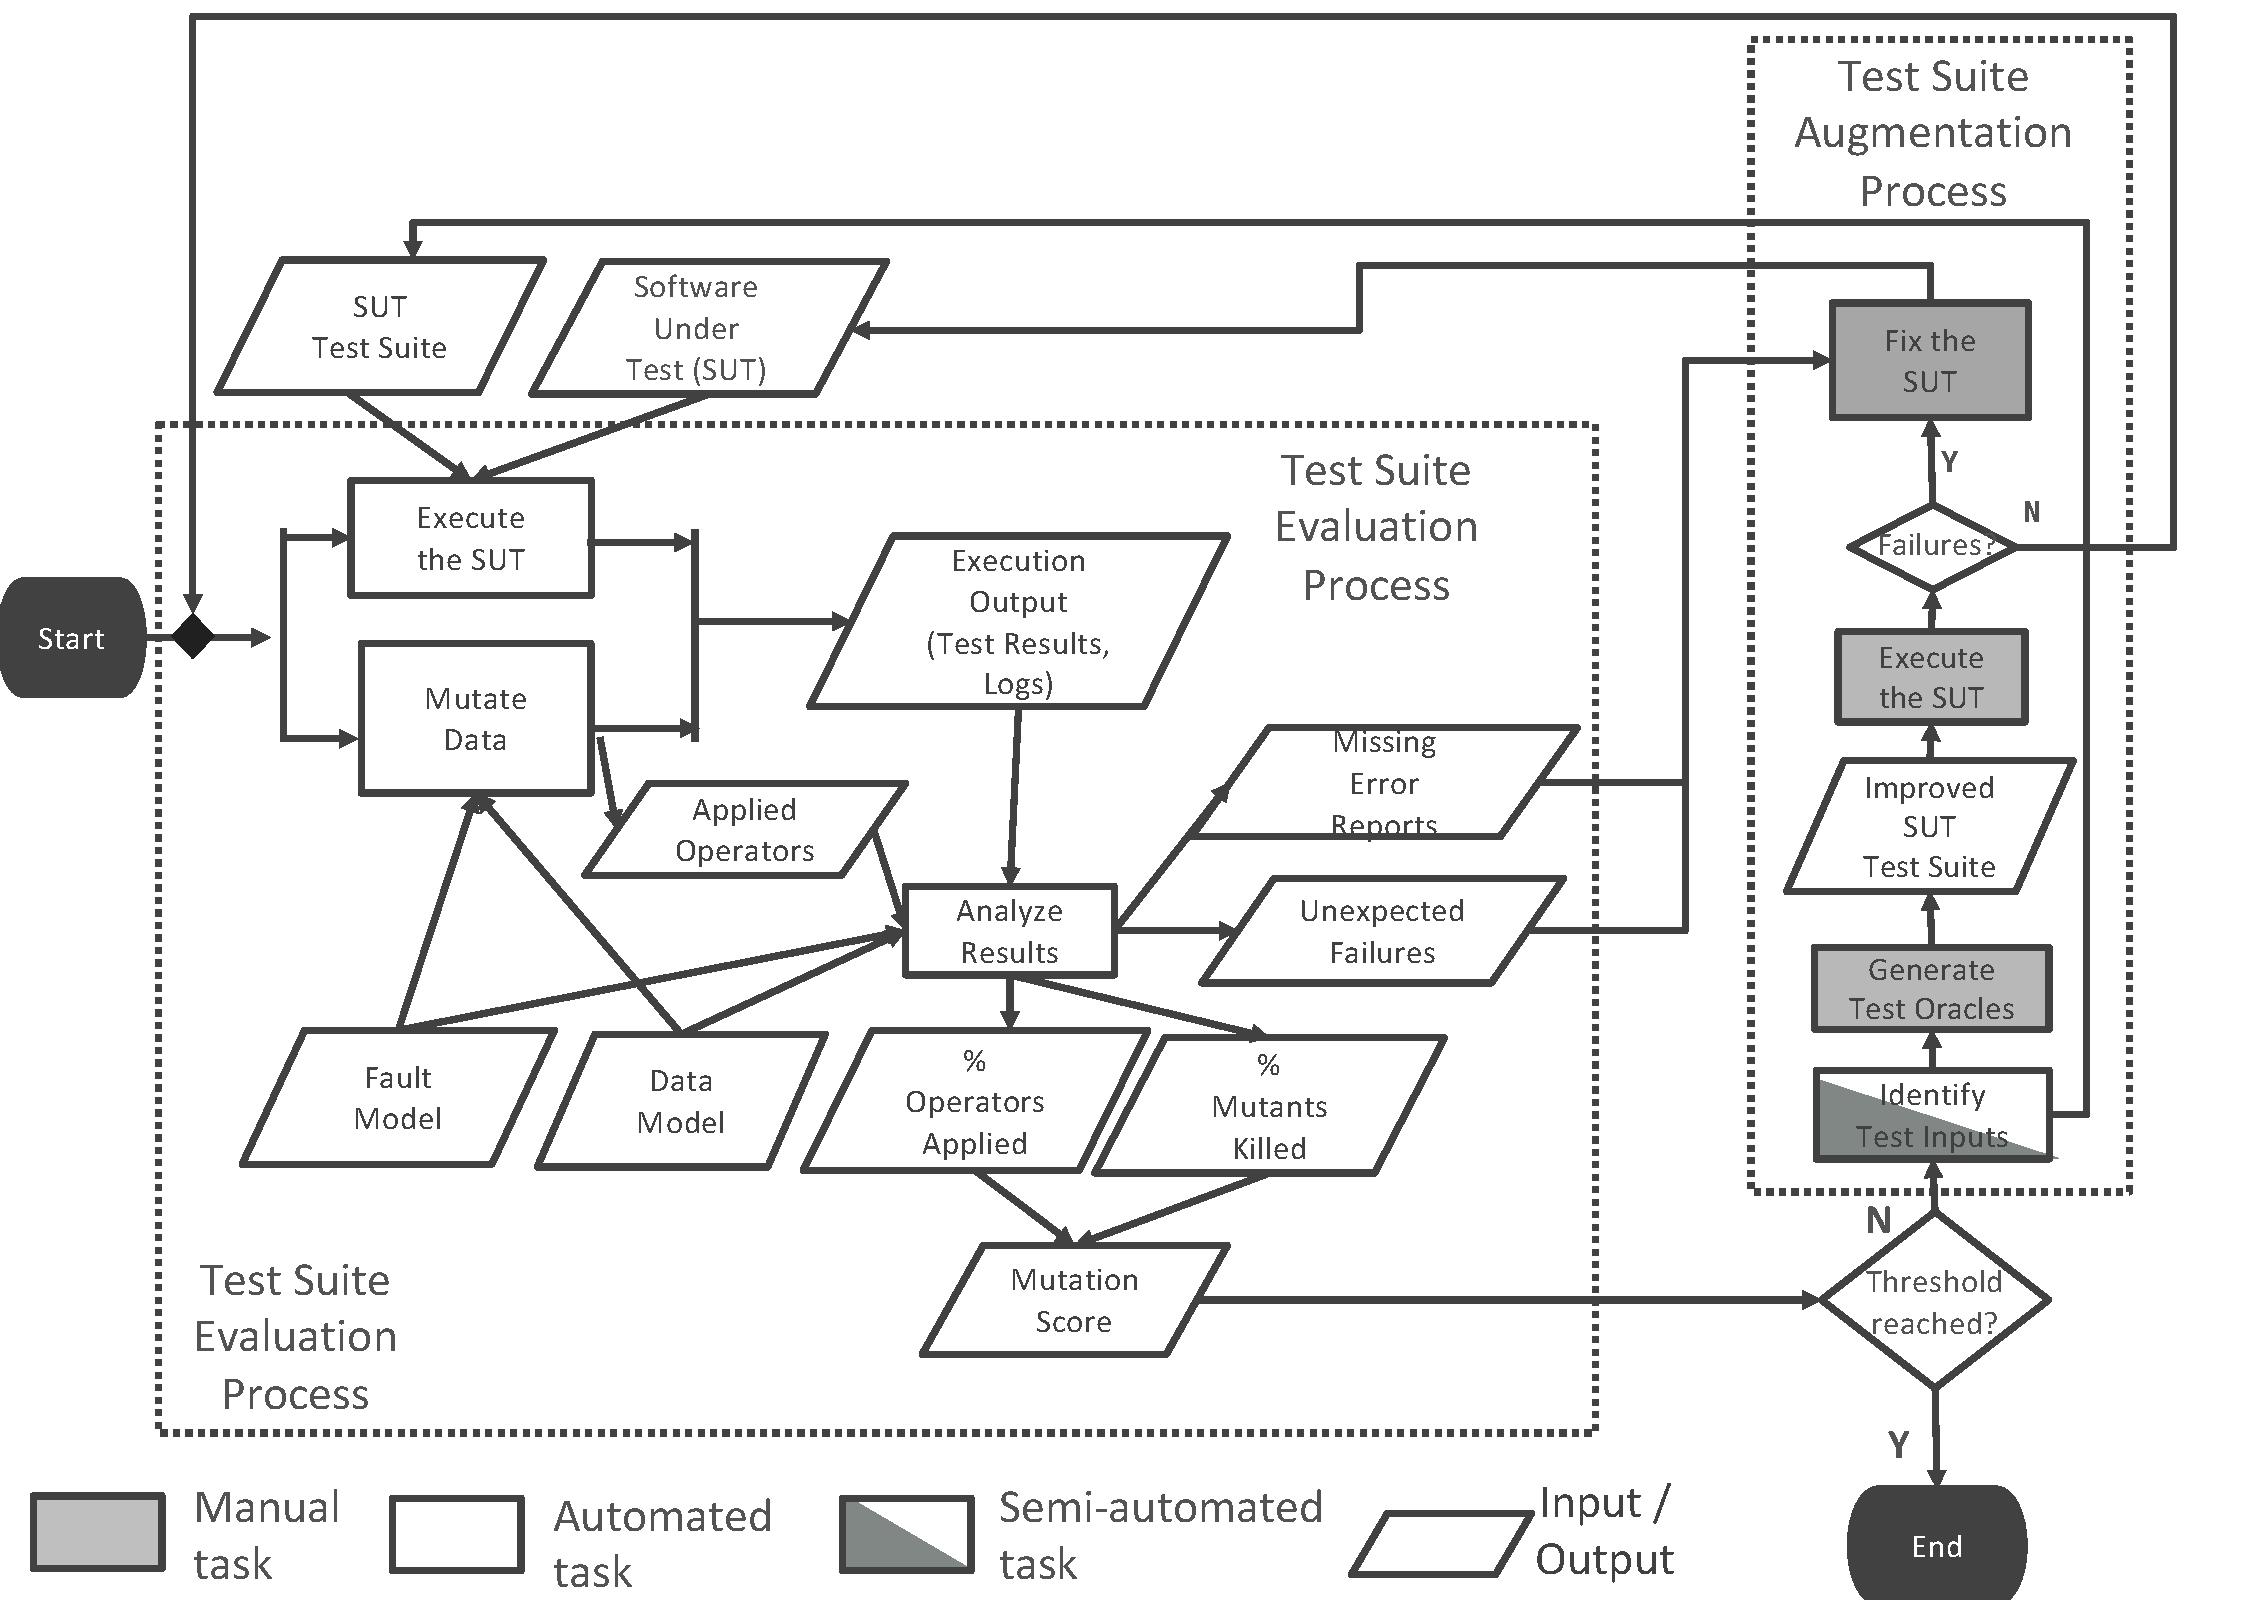
\includegraphics[width=\textwidth]{images/dataProcess}
		\caption{Data-driven Mutation Testing Process.}
		\label{fig:data:process}
	\end{figure}



This Chapter is a first attempt towards the formalization of a test suite assessment process based on the adoption of fault injection techniques that alter the data processed by software components; we refer to this process as \emph{data-driven mutation testing}. 
Data-driven mutation testing aims to assess test suites by simulating software faults that affect the data produced, received, or exchanged by the software and its components.
It is based on a fault model capturing the type of data fault that might affect the system, based on domain knowledge and engineers experience~\cite{di2015generating}.
Data-driven mutation testing has the following objectives:
(i) ensure that the test suite is capable of detecting software faults that affect the data processed by the software components 
(e.g., we expect a test suite to fail in case the data exchanged by two components contains invalid values)
(ii) ensure that the test suite exercises enough software behaviours to discover all the possible faults that may affect the data produced by the system
(i.e., it should be possible to alter the processed data to generate faulty data matching the fault model).

Figure \ref{fig:data:process} shows the reference code-driven mutation testing process that will be considered in this book. The process is based on two main sub-processes, \emph{test suite evaluation} and \emph{test suite augmentation}, which are described in Sections~\ref{sec:data:test_suite_evaluation}~and~\ref{sec:data:test_suite_augmentation}, respectively. Differently from the code-driven mutation testing process introduced in Section~\ref{sec:process}, the data-driven mutation testing process has not been formalized by existing software testing literature. 
Techniques to inject data faults in the data processed by software systems have been applied mostly to test software systems (e.g., to determine if the software is robust against errors in the data being processed) but not to assess the quality of test suites.
For systems, or components, exchanging structured data (e.g., message sequences), a data fault may consist of either an invalid data structure (i.e., a structure that does not respect the data model of the system) or an illegal data value.
For systems, or components, processing signals, a data fault may result in signals that do not respect the characteristics observed in the original signal. Example of signal features are value, derivative, second derivative~\cite{Matinnejad19}.

\subsection{Test Suite Evaluation} % (fold)
\label{sec:data:test_suite_evaluation}

The test suite evaluation process consists of three activities \emph{Execute the SUT}, \emph{Mutate Data},  and \emph{Analyze Results}.
The activity \emph{Execute the SUT} indicates that the SUT is executed against its automated test suite. 
The activity \emph{Mutate Data} concerns the automated modification of either the data received by the software, the data produced by the software, or the data exchanged by software components.
In Figure~\ref{fig:data:process}, the activity \emph{Mutate Data} is executed in parallel to the activity \emph{Execute the SUT} since data modification should occur at runtime during test cases execution, to simulate software faults affecting the data processed by the software.

The activity \emph{Mutate Data} requires a data model that captures the characteristics and structure of the data to be mutated. 
For example, the data model is used to load a stream of bytes in structured form (e.g., an instance of a given data structure), which is necessary to drive the data mutation. 
The activity \emph{Mutate Data} should be driven by a fault model that specifies the set of mutation operators to apply~\cite{di2015generating}. 
The data model enables engineers to minimize the presence of equivalent mutants.
%The data model may capture the relation between inputs and outputs of the system


The activity \emph{Analyze Results} processes all the output generated during test case execution.
The collected output includes the result of test cases execution (i.e., the list of test cases that either passed or failed) and the logs generated by the SUT during testing.
Logs are used to verify  the internal behaviour of the SUT that might not be reflected in the test cases results.
This is made necessary by the robustness features implemented in the software. For example, a system that implement a robust communication protocol might simply trigger the resending of packets affected by errors thus avoiding failures. In this case, engineers may need to inspect the log to determine if the robustness features had been triggered.

The data-driven mutation testing process may directly help engineers to identify faults. Indeed,
in the case of \emph{Missing Error Reports} or \emph{Unexpected Failures }(e.g, crashes), engineers should fix the system.

The qualify of the test suite is evaluated in terms of percentage of expected failures observed (i.e., mutants being killed) and percentage of mutation operators applied. The former enables data-driven mutation to achieve the objective (i) indicated above, the latter objective (ii). 
The identification of both the two types of information should is enabled by knowing the data, the fault model, and the mutations performed. 
More precisely, the fault model should specify which operators are expected to lead to test failures fail in the presence of data faults, and which should lead to error messages in the log. 
The list of applied mutation operators should instead enable engineers to determine if all the available mutation operators have been applied or not.






% subsection test_suite_evaluation (end)

\subsection{Test Suite Augmentation} % (fold)
\label{sec:data:test_suite_augmentation}

The test suite augmentation process concerns the definition of test cases that kill live mutants.
It consists of four activities \emph{Identify Test Inputs}, \emph{Generate Test Oracles}, \emph{Execute the SUT}, \emph{Fix the SUT}. The first two activities concern the definition of new test cases.
The third activity, i.e., the execution of the SUT, enables engineers to determine if the newly defined test cases spot faults not identified by the original test suite. 
Finally, the repair of the SUT (i.e., activity \emph{Fix the SUT}) is performed in the case of test failures.
In this book we focus on the techniques that can be applied to automate the first two activities (i.e., \emph{Identify Test Inputs}, and \emph{Generate Test Oracles}).
 
The identification of test inputs has the objective of identifying inputs for the SUT that make the SUT produce an output that is different than the one produced by one of the mutants not killed by the existing test suite.


Section~\ref{sec:data:testGeneration} provides an overview of approaches for the automated generation of test cases.

% subsection test_suite_augmentation (end)
